Redux es un administrador de estado predecible para aplicaciones JavaScript basado en el patrón de diseño Flux. A medida que una aplicación crece, se hace difícil mantenerla organizada y mantener el flujo de datos. Redux resuelve este problema administrando el estado de la aplicación con un único objeto global llamado Redux Store. Los principios fundamentales de Redux ayudan a mantener la coherencia en toda la aplicación, lo que facilita la depuración y las pruebas. Redux se puede conectar con cualquier biblioteca de JavaScript. Sin embargo, funciona muy bien con ReactJS debido a su naturaleza funcional.
\vspace{0.8cm}

Redux ayuda a separar el estado de la aplicación, crea un almacén global que reside en el nivel superior de una aplicación y alimenta con el estado a todos los componentes internos. A diferencia de Flux, Redux no tiene múltiples objetos de almacenamiento. El estado completo de la aplicación está dentro de un objeto, y potencialmente podría intercambiar la capa de vista con otra biblioteca con el almacenamiento intacto.

\subsubsection{Redux/Flux}
Redux adoptó un gran número de restricciones de la arquitectura Flux: las acciones encapsulan la información para que el Redux Reducer actualice el estado de manera determinista, el estado es un Redux Store singleton. El despachador de Flux único se reemplaza con múltiples Redux Reducers pequeños que recogen información de las acciones y la `reducen' a un nuevo estado que luego se guarda en el Redux Store. Cuando se cambia el estado en el Store, la Vista según la suscripción recibe propiedades llamadas props.
\vspace{0.8cm}

\begin{figure}[H]
  \centering
  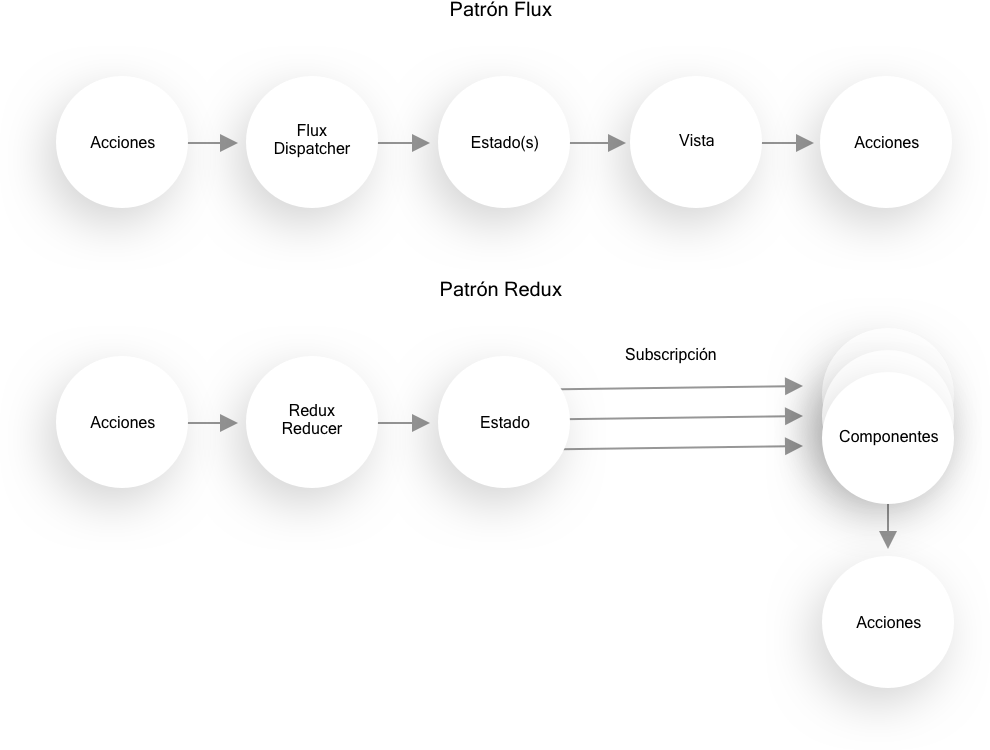
\includegraphics[width=0.9\textwidth]{flux-redux}
  \caption{Comparación Flux/Redux.}
\end{figure}
\vspace{0.8cm}

Para trabajar con Redux se necesitan tres cosas:
\begin{itemize}
  \item Actions (acciones): estos son objetos que deben tener dos propiedades, una que describe el tipo de acción y otra que describe lo que se debe cambiar en el estado de la aplicación.

  \item Reducers (reductores): son funciones que implementan el comportamiento de las acciones. Cambian el estado de la aplicación, en función de la descripción de la acción y la descripción del cambio de estado.

  \item Store (almacén): reúne las acciones y los reducers, manteniendo y cambiando el estado de toda la aplicación; solo hay una store.
\end{itemize}

\subsubsection{Redux Store}
Redux Store contiene un objeto del estado global de la aplicación. Esta actualiza el estado y notifica los componentes suscritos.
\vspace{0.8cm}

\lstinputlisting[style=ES6, caption=Fragmento de código para inicializar el Redux Store]{code/redux-store.js}

\subsubsection{Redux Reducer}
Un Redux Reducer es solo una función pura de JavaScript. Recibe dos parámetros: el estado actual y la acción. Una función pura es aquella que devuelve exactamente la misma salida para la entrada dada. El estado es el objeto Redux Store completo, la acción es el objeto despachado con un tipo requerido y un payload opcional.
\vspace{0.8cm}

\lstinputlisting[style=ES6, caption=Fragmento de código del reducer común de la app]{code/redux-reducer.js}

\subsubsection{Acciones Redux}
La única forma de cambiar el estado es enviando una señal al Store. Esta señal es una acción. Entonces "despachar una acción" significa enviar una señal a Redux Store.
\vspace{0.8cm}

\lstinputlisting[style=ES6, caption=Fragmento de una acción que actualiza el estado]{code/redux-action.js}

Este es un modelo conveniente y directo para estructurar datos en una aplicación y presentarlos en el cliente. La aplicación tiene un estado raíz. Un cambio de estado desencadena actualizaciones de vista. Solo las funciones especiales pueden modificar el estado. Una interacción del usuario activa estas funciones especiales de cambio de estado. Solo se produce un cambio a la vez. Esto significa que el estado central no puede desencadenar ninguna otra acción. Solo una entrada del usuario puede desencadenar otra acción \cite{mukhiya}.